\section{NUV Imaging TA verification}\label{sec:NimVER}

\subsection{Verifying the \tacq{IMAGE} WCA-to-SA Offsets.}\label{subsec:WCA2SAVER}

These results can be combined to show the measured offsets of PSA+MIRRORB, BOA+MIRRORA, and BOA+MIRRORB when compared to the initial PSA+MIRRORA \tacq{IMAGE} of Visit `A2' of P14035. These results are shown in Table~\ref{tab:ai}.
Combined offsets from PSA+MIRRORA are provided in both NUV pixels (p) and in arcseconds (\arcsec).
\clearpage
The results of P13972 and P14035 show that, for \tacq{IMAGE}s :
\footnotesize
\begin{itemize}
\item PSA+MIRRORA is aligned with PSA+MIRRORB to [AD, XD] $\le$ [0.022, 0.007]\arcsec\ (14035, Visit `A2')
\item PSA+MIRRORB is aligned with BOA+MIRRORA to [AD, XD] $\le$ [0.023, 0.100]\arcsec\ (13972, Visit `01')
\item BOA+MIRRORA is aligned with BOA+MIRRORB to [AD, XD] $\le$ [0.022, 0.024]\arcsec\ (13972, Visit `02')
\end{itemize}

\begin{deluxetable}{|r|r|r|r|r|r|}
\tabcolsep 10pt
\tabletypesize{\footnotesize}
\tablecolumns{6}
\tablewidth{0 pt}
\tablecaption{\tacq{IMAGE} WCA-to-SA offsets from PSA+MIRRORA\label{tab:ai}}
\tablehead{\colhead{Aperture}&\colhead{MIRROR}&\colhead{AD Offset} & \colhead{XD Offset} & \colhead{AD Offset}& \colhead{XD Offset}\\
\colhead{}&\colhead{}&\colhead{(\arcsec)} & \colhead{(\arcsec)} & \colhead{(p)} & \colhead{(p)}\\
}
\startdata
\hline
PSA & B & 0.021 &-0.049 & 0.298 & 0.893\\
BOA & A & 0.010 & 0.060 & 0.425 & 2.550\\
BOA & B & 0.036 & 0.070 & 1.530 & 2.975 \\
\hline
\enddata
\end{deluxetable}

\vspace{-0.3cm}
\section{WCA Lamp Images (aka, Lamp Family Portrait) \label{sec:family_portrait} }
\vspace{-0.3cm}

\begin{figure}[htb]
\vspace{1.3cm}
\centering
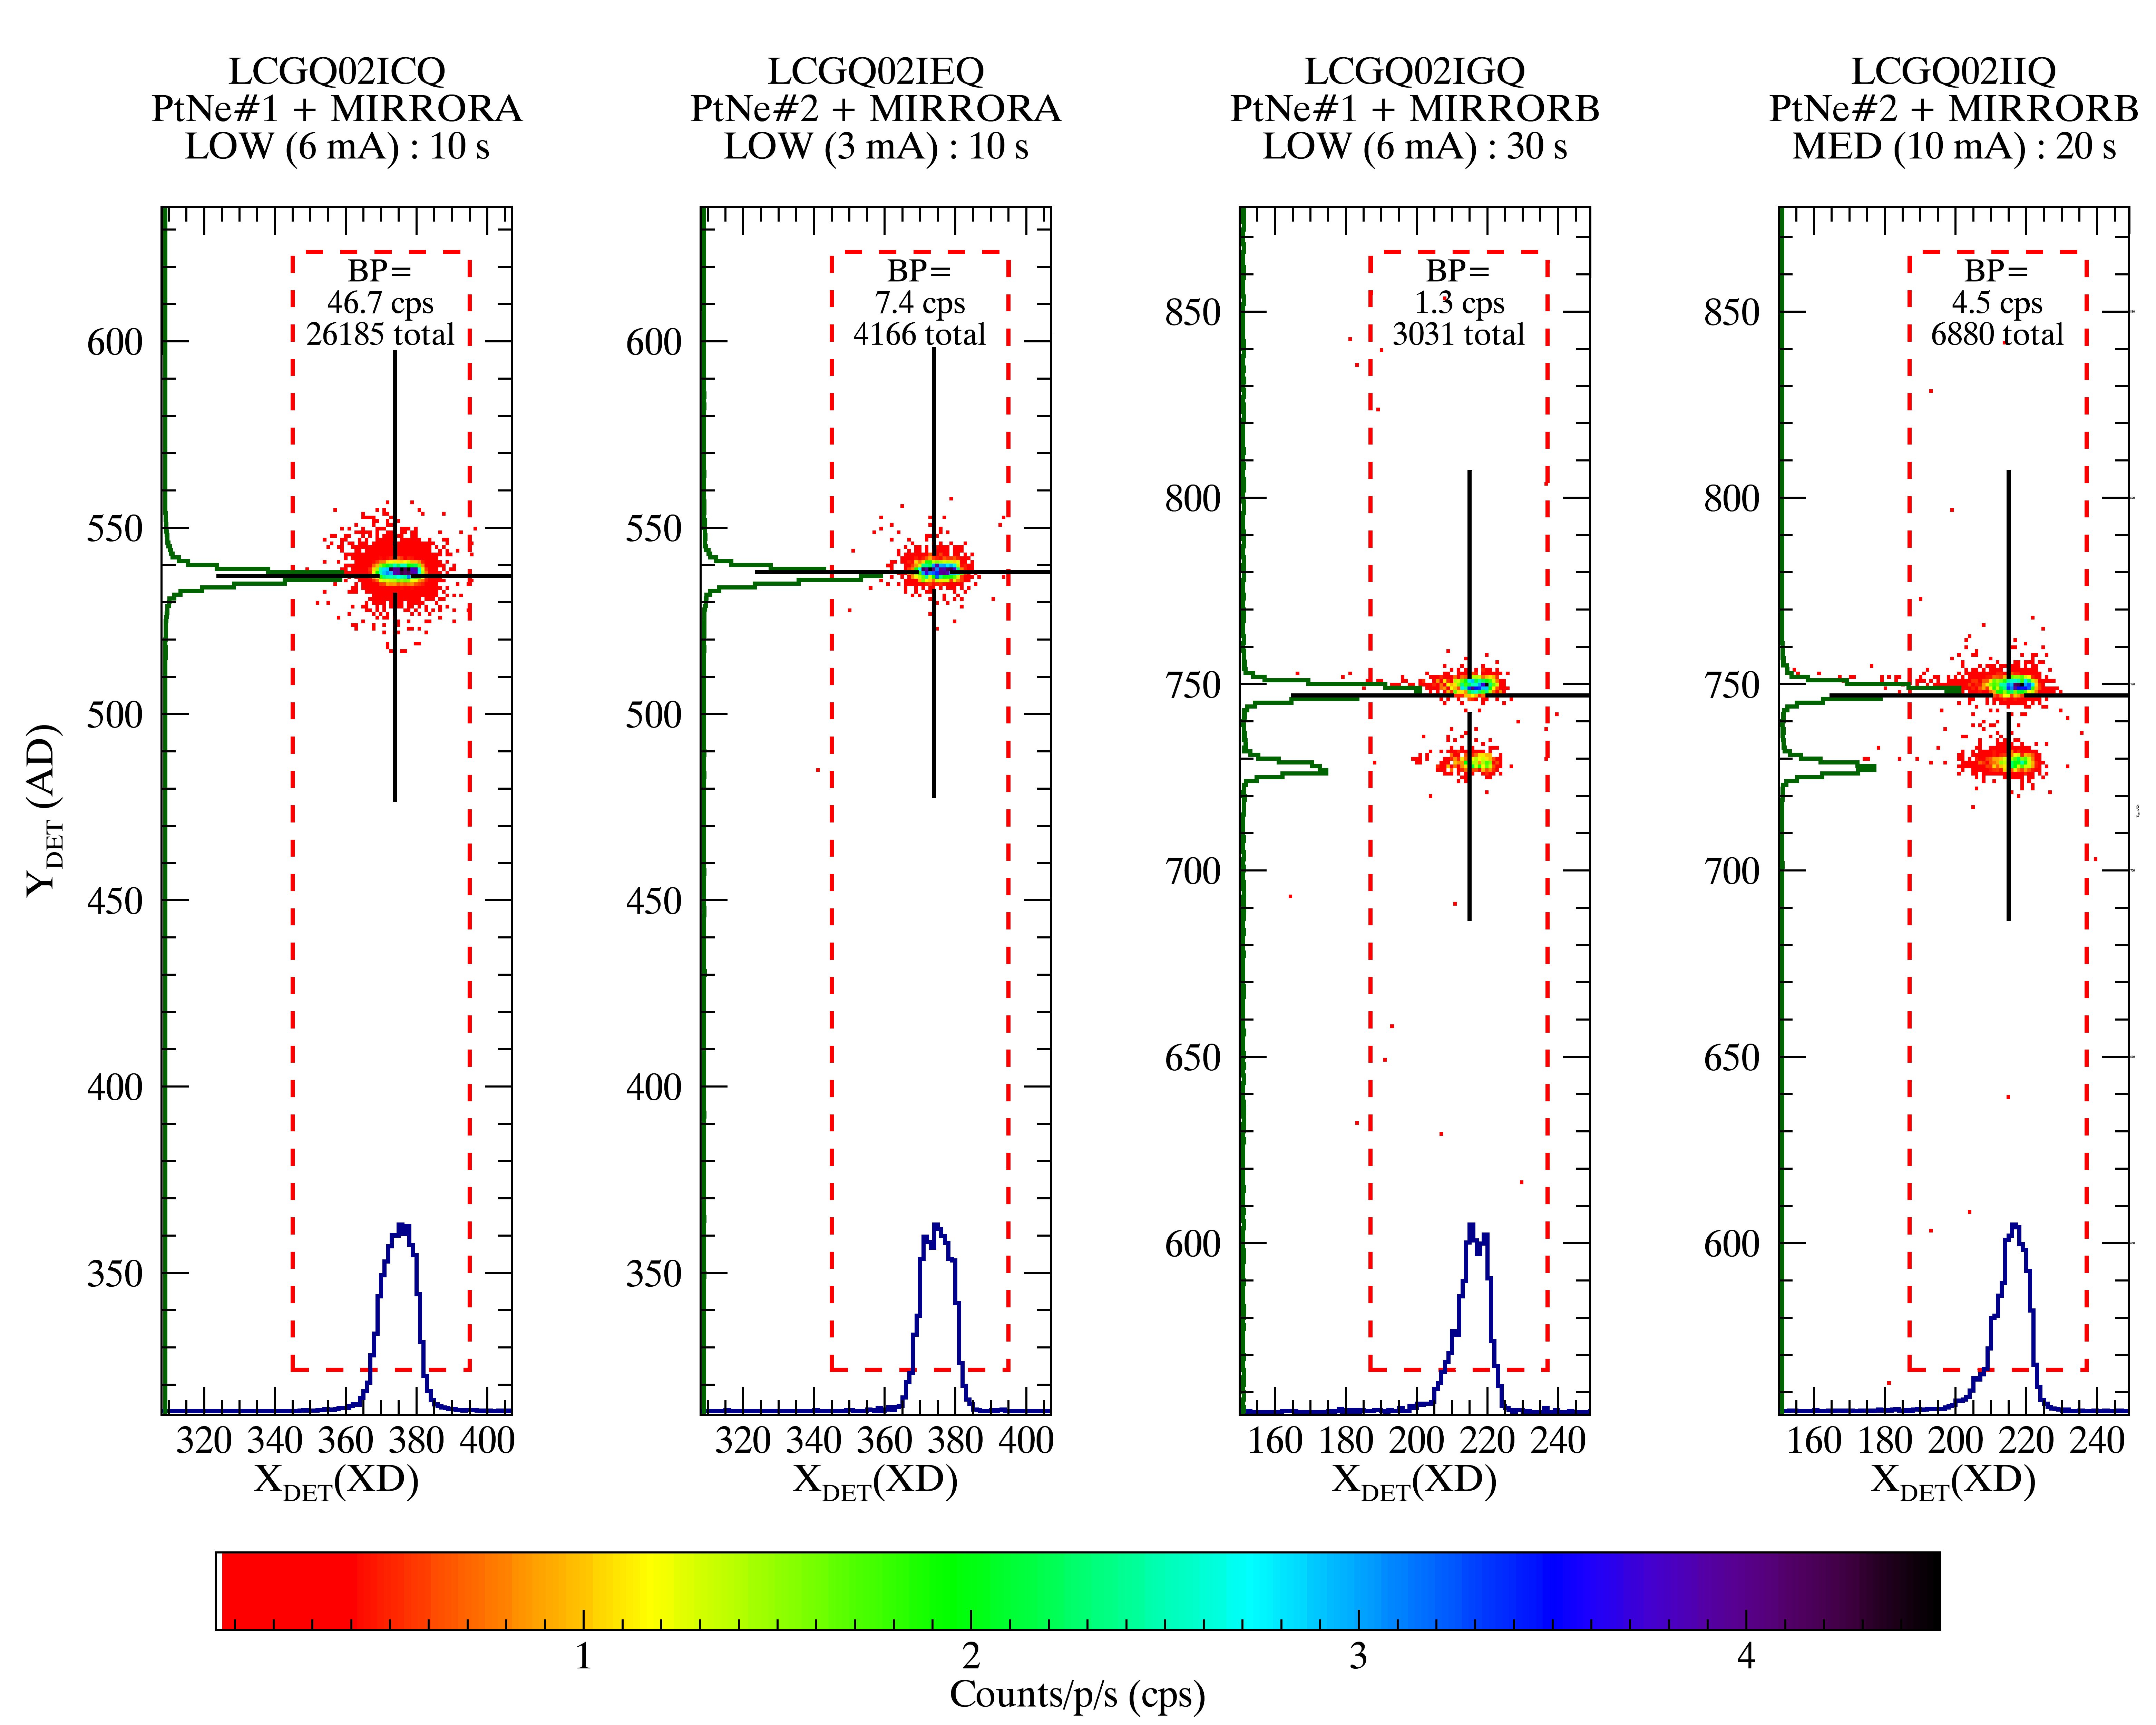
\includegraphics[width=\textwidth]{png/C21_13526_FP.png}
\caption{These four panels show a `family portrait' of the available COS PtNe Lamp + MIRROR combinations possible with \tacq{IMAGE}. Panel titles give the lamp and mirror combination, along with the current setting (in milli-amps, mA) and the exposure times in this program.
These images are in `detector' coordinates, as used on-board COS.
The images show the observed counts/pixel/s (cps) as given by the colorbar on the bottom.
The \textcolor{red}{red} dashed boxes show the Cycle~24 \tacq{IMAGE}~WCA subarrays. At the top of the subarrays, text provides the count rate in the brightest pixel (BP) in units of counts per second per NUV MAMA pixel (cps).
The \textcolor{blue}{blue} histogram on the bottom edge shows the cross-dispersion (XD) lamp profile in detector `X' coordinates, while
the \textcolor{green}{green} histogram on the left edge shows the along-dispersion (AD) lamp profile in detector `Y' coordinates.
The cross-hairs show the median location of the given configurations' lamp events within the TA subarray.
PtNe\#2 lamp was used for all \tacq{IMAGE}s~ during Cycle~24, and was operated at LOW current (6~mA) for those using MIRRORA and MEDium current (10~mA) for those using MIRRORB.
}
\label{fig:FP}
\vspace{1.3cm}
\end{figure}

\begin{figure}[htb]
\noindent\includegraphics*[width=0.795\linewidth]{png/C22_13972_FP.png}
\caption{Cycle~22 PtNe Lamp `Family Portrait'' \ref{fig:FG21}}
\end{figure}

\begin{figure}[htb]
\noindent\includegraphics*[width=0.795\linewidth]{png/C23_14440_FP.png}
\caption{Cycle~23 PtNe Lamp `Family Portrait'' \ref{fig:FG22}}
\end{figure}

\begin{figure}[htb]
\noindent\includegraphics*[width=0.795\linewidth]{png/C24_14857_FP.png}
\caption{Cycle 24 PtNe Lamp `Family Portrait'' \ref{fig:FG21}}
\end{figure}

\begin{figure}[htb]
\noindent\includegraphics*[width=0.795\linewidth]{png/C24_14857_Error_vs_lampSN.png}
\caption{Cycle~24 PtNe Lamp `Family Portrait'' \ref{fig:FG24}}
\end{figure}
\clearpage
\subsection{Verifying the \tacq{PEAKXD} WCA-to-PSA Offsets.} \label{subsec:acqpeakxd}

\tiny
\begin{deluxetable}{lclcccr}
\tablewidth{0pt}
\tabcolsep 10pt
\tablecolumns{7}
\tabletypesize{\footnotesize}
\tablecaption{COS Cycle~24 TA Monitoring Results Summary\label{tab:table_one}}
\tablehead{
\colhead{ACQ} & \colhead{COS} & \colhead{Optical} & \colhead{Direction} & \colhead{Measured Offset\tablenotemark{b}} & \colhead{Requirement} & \colhead{Goal}\\
\colhead{Mode} & \colhead{Channel} & \colhead{Configuration} & \colhead{AD or XD} & \colhead{mas\tablenotemark{a}} & \colhead{mas\tablenotemark{a}} & \colhead{mas\tablenotemark{a}}\\
}
\startdata
\hline
IMAGE	&	NUV	&	PSA+MIRRORA	&	AD	&	20$\pm$14	&	41--105	&	40\\
IMAGE	&	NUV	&	PSA+MIRRORB	&	AD	&	10$\pm$14	&	41--105	&	40\\
IMAGE	&	NUV	&	BOA+MIRRORA	&	AD	&	20$\pm$14	&	41--105	&	40\\
IMAGE	&	NUV	&	BOA+MIRRORB	&	AD	&	15$\pm$14	&	41--105	&	40\\
\hline
IMAGE	&	NUV	&	PSA+MIRRORA	&	XD	&	75$\pm$14	&	300		&	100\\
IMAGE	&	NUV	&	PSA+MIRRORB	&	XD	&	20$\pm$14	&	300		&	100\\
IMAGE	&	NUV	&	BOA+MIRRORA	&	XD	&	95$\pm$14	&	300		&	100\\
IMAGE	&	NUV	&	BOA+MIRRORB	&	XD	&	12$\pm$14	&	300		&	100\\
\hline
PEAKXD	&	NUV	&	G185M		&	XD	&	 70$\pm$17		&	300		&	100\\
PEAKXD	&	NUV	&	G225M		&	XD	&	 60$\pm$17		&	300		&	100\\
PEAKXD	&	NUV	&	G285M		&	XD	&	 20$\pm$17		&	300		&	100\\
PEAKXD	&	NUV	&	G230L		&	XD	&	 20$\pm$17		&	300		&	100\\
PEAKXD	&	FUVA	&	G130M		&	XD	&	-30$\pm$71		&	300		&	100\\
PEAKXD	&	FUVA	&	G160M		&	XD	&	-20$\pm$71		&	300		&	100\\
PEAKXD	&	FUVA	&	G140L		&	XD	&	-170$\pm$71		&	300		&	100\\
\hline
\enddata
\tablenotetext{a}{1 mas = 1 milli-arcsecond.}
\tablenotetext{b}{The quoted error bars are associated with a 0.5 uncertainty when measuring the integer WCA coordinate,
and 1/3 of an NUV pixel when using the \tacq{IMAGE}~checkbox centering algorithm. Added in quadrature, the approximate
\tacq{IMAGE}~measurement error is $\approx 0.6$ NUV pixels, or 14 mas.
Each \tacq{PEAKXD}~ WCA-to-SA measurement contains an error estimate of $\sqrt2 * 0.5 $ times the plate scale of the detector in use
(one half pixel or digital-element uncertainty for each measurement of an integer quantity).
For the NUV channel, this is 23.5 mas/p or $\sqrt2 * 0.5 * 23.5 = 17$ mas.
For the FUV channel, this is $\approx \sqrt2 * 0.5 * 100 \approx 71$ mas.}
\end{deluxetable}
